\documentclass[]{article}
\usepackage{lmodern}
\usepackage{amssymb,amsmath}
\usepackage{ifxetex,ifluatex}
\usepackage{fixltx2e} % provides \textsubscript
\ifnum 0\ifxetex 1\fi\ifluatex 1\fi=0 % if pdftex
  \usepackage[T1]{fontenc}
  \usepackage[utf8]{inputenc}
\else % if luatex or xelatex
  \ifxetex
    \usepackage{mathspec}
  \else
    \usepackage{fontspec}
  \fi
  \defaultfontfeatures{Ligatures=TeX,Scale=MatchLowercase}
\fi
% use upquote if available, for straight quotes in verbatim environments
\IfFileExists{upquote.sty}{\usepackage{upquote}}{}
% use microtype if available
\IfFileExists{microtype.sty}{%
\usepackage{microtype}
\UseMicrotypeSet[protrusion]{basicmath} % disable protrusion for tt fonts
}{}
\usepackage[margin=1in]{geometry}
\usepackage{hyperref}
\hypersetup{unicode=true,
            pdftitle={Storm.rmd},
            pdfborder={0 0 0},
            breaklinks=true}
\urlstyle{same}  % don't use monospace font for urls
\usepackage{color}
\usepackage{fancyvrb}
\newcommand{\VerbBar}{|}
\newcommand{\VERB}{\Verb[commandchars=\\\{\}]}
\DefineVerbatimEnvironment{Highlighting}{Verbatim}{commandchars=\\\{\}}
% Add ',fontsize=\small' for more characters per line
\usepackage{framed}
\definecolor{shadecolor}{RGB}{248,248,248}
\newenvironment{Shaded}{\begin{snugshade}}{\end{snugshade}}
\newcommand{\KeywordTok}[1]{\textcolor[rgb]{0.13,0.29,0.53}{\textbf{#1}}}
\newcommand{\DataTypeTok}[1]{\textcolor[rgb]{0.13,0.29,0.53}{#1}}
\newcommand{\DecValTok}[1]{\textcolor[rgb]{0.00,0.00,0.81}{#1}}
\newcommand{\BaseNTok}[1]{\textcolor[rgb]{0.00,0.00,0.81}{#1}}
\newcommand{\FloatTok}[1]{\textcolor[rgb]{0.00,0.00,0.81}{#1}}
\newcommand{\ConstantTok}[1]{\textcolor[rgb]{0.00,0.00,0.00}{#1}}
\newcommand{\CharTok}[1]{\textcolor[rgb]{0.31,0.60,0.02}{#1}}
\newcommand{\SpecialCharTok}[1]{\textcolor[rgb]{0.00,0.00,0.00}{#1}}
\newcommand{\StringTok}[1]{\textcolor[rgb]{0.31,0.60,0.02}{#1}}
\newcommand{\VerbatimStringTok}[1]{\textcolor[rgb]{0.31,0.60,0.02}{#1}}
\newcommand{\SpecialStringTok}[1]{\textcolor[rgb]{0.31,0.60,0.02}{#1}}
\newcommand{\ImportTok}[1]{#1}
\newcommand{\CommentTok}[1]{\textcolor[rgb]{0.56,0.35,0.01}{\textit{#1}}}
\newcommand{\DocumentationTok}[1]{\textcolor[rgb]{0.56,0.35,0.01}{\textbf{\textit{#1}}}}
\newcommand{\AnnotationTok}[1]{\textcolor[rgb]{0.56,0.35,0.01}{\textbf{\textit{#1}}}}
\newcommand{\CommentVarTok}[1]{\textcolor[rgb]{0.56,0.35,0.01}{\textbf{\textit{#1}}}}
\newcommand{\OtherTok}[1]{\textcolor[rgb]{0.56,0.35,0.01}{#1}}
\newcommand{\FunctionTok}[1]{\textcolor[rgb]{0.00,0.00,0.00}{#1}}
\newcommand{\VariableTok}[1]{\textcolor[rgb]{0.00,0.00,0.00}{#1}}
\newcommand{\ControlFlowTok}[1]{\textcolor[rgb]{0.13,0.29,0.53}{\textbf{#1}}}
\newcommand{\OperatorTok}[1]{\textcolor[rgb]{0.81,0.36,0.00}{\textbf{#1}}}
\newcommand{\BuiltInTok}[1]{#1}
\newcommand{\ExtensionTok}[1]{#1}
\newcommand{\PreprocessorTok}[1]{\textcolor[rgb]{0.56,0.35,0.01}{\textit{#1}}}
\newcommand{\AttributeTok}[1]{\textcolor[rgb]{0.77,0.63,0.00}{#1}}
\newcommand{\RegionMarkerTok}[1]{#1}
\newcommand{\InformationTok}[1]{\textcolor[rgb]{0.56,0.35,0.01}{\textbf{\textit{#1}}}}
\newcommand{\WarningTok}[1]{\textcolor[rgb]{0.56,0.35,0.01}{\textbf{\textit{#1}}}}
\newcommand{\AlertTok}[1]{\textcolor[rgb]{0.94,0.16,0.16}{#1}}
\newcommand{\ErrorTok}[1]{\textcolor[rgb]{0.64,0.00,0.00}{\textbf{#1}}}
\newcommand{\NormalTok}[1]{#1}
\usepackage{graphicx,grffile}
\makeatletter
\def\maxwidth{\ifdim\Gin@nat@width>\linewidth\linewidth\else\Gin@nat@width\fi}
\def\maxheight{\ifdim\Gin@nat@height>\textheight\textheight\else\Gin@nat@height\fi}
\makeatother
% Scale images if necessary, so that they will not overflow the page
% margins by default, and it is still possible to overwrite the defaults
% using explicit options in \includegraphics[width, height, ...]{}
\setkeys{Gin}{width=\maxwidth,height=\maxheight,keepaspectratio}
\IfFileExists{parskip.sty}{%
\usepackage{parskip}
}{% else
\setlength{\parindent}{0pt}
\setlength{\parskip}{6pt plus 2pt minus 1pt}
}
\setlength{\emergencystretch}{3em}  % prevent overfull lines
\providecommand{\tightlist}{%
  \setlength{\itemsep}{0pt}\setlength{\parskip}{0pt}}
\setcounter{secnumdepth}{0}
% Redefines (sub)paragraphs to behave more like sections
\ifx\paragraph\undefined\else
\let\oldparagraph\paragraph
\renewcommand{\paragraph}[1]{\oldparagraph{#1}\mbox{}}
\fi
\ifx\subparagraph\undefined\else
\let\oldsubparagraph\subparagraph
\renewcommand{\subparagraph}[1]{\oldsubparagraph{#1}\mbox{}}
\fi

%%% Use protect on footnotes to avoid problems with footnotes in titles
\let\rmarkdownfootnote\footnote%
\def\footnote{\protect\rmarkdownfootnote}

%%% Change title format to be more compact
\usepackage{titling}

% Create subtitle command for use in maketitle
\newcommand{\subtitle}[1]{
  \posttitle{
    \begin{center}\large#1\end{center}
    }
}

\setlength{\droptitle}{-2em}

  \title{Storm.rmd}
    \pretitle{\vspace{\droptitle}\centering\huge}
  \posttitle{\par}
    \author{}
    \preauthor{}\postauthor{}
    \date{}
    \predate{}\postdate{}
  

\begin{document}
\maketitle

\section{Health and Economic Impact of Weather Events in the
US}\label{health-and-economic-impact-of-weather-events-in-the-us}

Storms and other severe weather events can cause both public health and
economic problems for communities and municipalities. Many severe events
can result in fatalities, injuries, and property damage, and preventing
such outcomes to the extent possible is a key concern.

This project involves exploring the U.S. National Oceanic and
Atmospheric Administration's (NOAA) storm database. This database tracks
characteristics of major storms and weather events in the United States,
including when and where they occur, as well as estimates of any
fatalities, injuries, and property damage.

\section{Synopsis}\label{synopsis}

The analysis on the storm event database revealed that tornadoes are the
most dangerous weather event to the population health. The second most
dangerous event type is the excessive heat. The economic impact of
weather events was also analyzed. Flash floods and thunderstorm winds
caused billions of dollars in property damages between 1950 and 2011.
The largest crop damage caused by drought, followed by flood and hails.

\section{Data Processing}\label{data-processing}

The analysis was performed on
\href{http://www.ncdc.noaa.gov/stormevents/ftp.jsp}{Storm Events
Database}, provided by \href{http://www.ncdc.noaa.gov/}{National
Climatic Data Center}. The data is from a comma-separated-value file
available
\href{https://d396qusza40orc.cloudfront.net/repdata\%2Fdata\%2FStormData.csv.bz2}{here}.
There is also some documentation of the data available
\href{https://d396qusza40orc.cloudfront.net/repdata\%2Fpeer2_doc\%2Fpd01016005curr.pdf}{here}.

The first step is to read the data into a data frame.

\begin{Shaded}
\begin{Highlighting}[]
\NormalTok{df <-}\StringTok{ }\KeywordTok{read.csv}\NormalTok{(}\KeywordTok{bzfile}\NormalTok{(}\StringTok{"/Users/jatin/Desktop/storm.bz2"}\NormalTok{))}
\end{Highlighting}
\end{Shaded}

Before the analysis, the data need some preprocessing. Event types don't
have a specific format. For instance, there are events with types
\texttt{Frost/Freeze}, \texttt{FROST/FREEZE} and
\texttt{FROST\textbackslash{}\textbackslash{}FREEZE} which obviously
refer to the same type of event.

\begin{Shaded}
\begin{Highlighting}[]
\CommentTok{# number of unique event types}
\KeywordTok{length}\NormalTok{(}\KeywordTok{unique}\NormalTok{(df}\OperatorTok{$}\NormalTok{EVTYPE))}
\end{Highlighting}
\end{Shaded}

\begin{verbatim}
## [1] 985
\end{verbatim}

\begin{Shaded}
\begin{Highlighting}[]
\CommentTok{# translate all letters to lowercase}
\NormalTok{event_types <-}\StringTok{ }\KeywordTok{tolower}\NormalTok{(df}\OperatorTok{$}\NormalTok{EVTYPE)}
\CommentTok{# replace all punct. characters with a space}
\NormalTok{event_types <-}\StringTok{ }\KeywordTok{gsub}\NormalTok{(}\StringTok{"[[:blank:][:punct:]+]"}\NormalTok{, }\StringTok{" "}\NormalTok{, event_types)}
\KeywordTok{length}\NormalTok{(}\KeywordTok{unique}\NormalTok{(event_types))}
\end{Highlighting}
\end{Shaded}

\begin{verbatim}
## [1] 874
\end{verbatim}

\begin{Shaded}
\begin{Highlighting}[]
\CommentTok{# update the data frame}
\NormalTok{df}\OperatorTok{$}\NormalTok{EVTYPE <-}\StringTok{ }\NormalTok{event_types}
\end{Highlighting}
\end{Shaded}

No further data preprocessing was performed although the event type
field can be processed further to merge event types such as
\texttt{tstm\ wind} and \texttt{thunderstorm\ wind}. After the cleaning,
as expected, the number of unique event types reduce significantly. For
further analysis, the cleaned event types are used.

\section{Dangerous Events with respect to Population
Health}\label{dangerous-events-with-respect-to-population-health}

To find the event types that are most harmful to population health, the
number of casualties are aggregated by the event type.

\begin{Shaded}
\begin{Highlighting}[]
\KeywordTok{library}\NormalTok{(dplyr)}
\end{Highlighting}
\end{Shaded}

\begin{verbatim}
## 
## Attaching package: 'dplyr'
\end{verbatim}

\begin{verbatim}
## The following objects are masked from 'package:stats':
## 
##     filter, lag
\end{verbatim}

\begin{verbatim}
## The following objects are masked from 'package:base':
## 
##     intersect, setdiff, setequal, union
\end{verbatim}

\begin{Shaded}
\begin{Highlighting}[]
\NormalTok{casual <-}\StringTok{ }\NormalTok{df}\OperatorTok\KeywordTok{group_by}\NormalTok{(EVTYPE)}\OperatorTok\KeywordTok{summarize}\NormalTok{(}\DataTypeTok{fatalities =} \KeywordTok{sum}\NormalTok{(FATALITIES),}
                                            \DataTypeTok{injuries =} \KeywordTok{sum}\NormalTok{(INJURIES))}

\CommentTok{# Find events that caused most death and injury}
\NormalTok{fatal_events <-}\StringTok{ }\KeywordTok{head}\NormalTok{(casual[}\KeywordTok{order}\NormalTok{(casual}\OperatorTok{$}\NormalTok{fatalities, }\DataTypeTok{decreasing =}\NormalTok{ T), ], }\DecValTok{10}\NormalTok{)}
\NormalTok{injury_events <-}\StringTok{ }\KeywordTok{head}\NormalTok{(casual[}\KeywordTok{order}\NormalTok{(casual}\OperatorTok{$}\NormalTok{injuries, }\DataTypeTok{decreasing =}\NormalTok{ T), ], }\DecValTok{10}\NormalTok{)}
\end{Highlighting}
\end{Shaded}

Top 10 events that caused largest number of deaths are

\begin{Shaded}
\begin{Highlighting}[]
\NormalTok{fatal_events[, }\KeywordTok{c}\NormalTok{(}\StringTok{"EVTYPE"}\NormalTok{, }\StringTok{"fatalities"}\NormalTok{)]}
\end{Highlighting}
\end{Shaded}

\begin{verbatim}
## # A tibble: 10 x 2
##    EVTYPE         fatalities
##    <chr>               <dbl>
##  1 tornado              5633
##  2 excessive heat       1903
##  3 flash flood           978
##  4 heat                  937
##  5 lightning             816
##  6 tstm wind             504
##  7 flood                 470
##  8 rip current           368
##  9 high wind             248
## 10 avalanche             224
\end{verbatim}

Top 10 events that caused most number of injuries are

\begin{Shaded}
\begin{Highlighting}[]
\NormalTok{injury_events[, }\KeywordTok{c}\NormalTok{(}\StringTok{"EVTYPE"}\NormalTok{, }\StringTok{"injuries"}\NormalTok{)]}
\end{Highlighting}
\end{Shaded}

\begin{verbatim}
## # A tibble: 10 x 2
##    EVTYPE            injuries
##    <chr>                <dbl>
##  1 tornado              91346
##  2 tstm wind             6957
##  3 flood                 6789
##  4 excessive heat        6525
##  5 lightning             5230
##  6 heat                  2100
##  7 ice storm             1975
##  8 flash flood           1777
##  9 thunderstorm wind     1488
## 10 hail                  1361
\end{verbatim}

\section{Economic Effects of Weather
Events}\label{economic-effects-of-weather-events}

To analyze the impact of weather events on the economy, available
property damage and crop damage reportings/estimates were used.

In the raw data, the property damage is represented with two fields, a
number \texttt{PROPDMG} in dollars and the exponent \texttt{PROPDMGEXP}.
Similarly, the crop damage is represented using two fields,
\texttt{CROPDMG} and \texttt{CROPDMGEXP}. The first step in the analysis
is to calculate the property and crop damage for each event.

\begin{Shaded}
\begin{Highlighting}[]
\NormalTok{exp_transform <-}\StringTok{ }\ControlFlowTok{function}\NormalTok{(e) \{}
    \CommentTok{# h -> hundred, k -> thousand, m -> million, b -> billion}
    \ControlFlowTok{if}\NormalTok{ (e }\OperatorTok\StringTok{ }\KeywordTok{c}\NormalTok{(}\StringTok{'h'}\NormalTok{, }\StringTok{'H'}\NormalTok{))}
        \KeywordTok{return}\NormalTok{(}\DecValTok{2}\NormalTok{)}
    \ControlFlowTok{else} \ControlFlowTok{if}\NormalTok{ (e }\OperatorTok\StringTok{ }\KeywordTok{c}\NormalTok{(}\StringTok{'k'}\NormalTok{, }\StringTok{'K'}\NormalTok{))}
        \KeywordTok{return}\NormalTok{(}\DecValTok{3}\NormalTok{)}
    \ControlFlowTok{else} \ControlFlowTok{if}\NormalTok{ (e }\OperatorTok\StringTok{ }\KeywordTok{c}\NormalTok{(}\StringTok{'m'}\NormalTok{, }\StringTok{'M'}\NormalTok{))}
        \KeywordTok{return}\NormalTok{(}\DecValTok{6}\NormalTok{)}
    \ControlFlowTok{else} \ControlFlowTok{if}\NormalTok{ (e }\OperatorTok\StringTok{ }\KeywordTok{c}\NormalTok{(}\StringTok{'b'}\NormalTok{, }\StringTok{'B'}\NormalTok{))}
        \KeywordTok{return}\NormalTok{(}\DecValTok{9}\NormalTok{)}
    \ControlFlowTok{else} \ControlFlowTok{if}\NormalTok{ (}\OperatorTok{!}\KeywordTok{is.na}\NormalTok{(}\KeywordTok{as.numeric}\NormalTok{(e))) }\CommentTok{# if a digit}
        \KeywordTok{return}\NormalTok{(}\KeywordTok{as.numeric}\NormalTok{(e))}
    \ControlFlowTok{else} \ControlFlowTok{if}\NormalTok{ (e }\OperatorTok\StringTok{ }\KeywordTok{c}\NormalTok{(}\StringTok{''}\NormalTok{, }\StringTok{'-'}\NormalTok{, }\StringTok{'?'}\NormalTok{, }\StringTok{'+'}\NormalTok{))}
        \KeywordTok{return}\NormalTok{(}\DecValTok{0}\NormalTok{)}
    \ControlFlowTok{else}\NormalTok{ \{}
        \KeywordTok{stop}\NormalTok{(}\StringTok{"Invalid exponent value."}\NormalTok{)}
\NormalTok{    \}}
\NormalTok{\}}
\end{Highlighting}
\end{Shaded}

\begin{Shaded}
\begin{Highlighting}[]
\NormalTok{prop_dmg_exp <-}\StringTok{ }\KeywordTok{sapply}\NormalTok{(df}\OperatorTok{$}\NormalTok{PROPDMGEXP, }\DataTypeTok{FUN=}\NormalTok{exp_transform)}
\NormalTok{df}\OperatorTok{$}\NormalTok{prop_dmg <-}\StringTok{ }\NormalTok{df}\OperatorTok{$}\NormalTok{PROPDMG }\OperatorTok{*}\StringTok{ }\NormalTok{(}\DecValTok{10} \OperatorTok{**}\StringTok{ }\NormalTok{prop_dmg_exp)}
\NormalTok{crop_dmg_exp <-}\StringTok{ }\KeywordTok{sapply}\NormalTok{(df}\OperatorTok{$}\NormalTok{CROPDMGEXP, }\DataTypeTok{FUN=}\NormalTok{exp_transform)}
\NormalTok{df}\OperatorTok{$}\NormalTok{crop_dmg <-}\StringTok{ }\NormalTok{df}\OperatorTok{$}\NormalTok{CROPDMG }\OperatorTok{*}\StringTok{ }\NormalTok{(}\DecValTok{10} \OperatorTok{**}\StringTok{ }\NormalTok{crop_dmg_exp)}
\end{Highlighting}
\end{Shaded}

\begin{Shaded}
\begin{Highlighting}[]
\CommentTok{# Compute the economic loss by event type}
\KeywordTok{library}\NormalTok{(dplyr)}

\NormalTok{econ_loss <-}\StringTok{ }\NormalTok{df}\OperatorTok\StringTok{ }\KeywordTok{group_by}\NormalTok{(EVTYPE)}\OperatorTok\KeywordTok{summarize}\NormalTok{(}\DataTypeTok{prop_dmg =} \KeywordTok{sum}\NormalTok{(prop_dmg),}
                                               \DataTypeTok{crop_dmg =} \KeywordTok{sum}\NormalTok{(crop_dmg))}

\CommentTok{# filter out events that caused no economic loss}
\NormalTok{econ_loss <-}\StringTok{ }\NormalTok{econ_loss[(econ_loss}\OperatorTok{$}\NormalTok{prop_dmg }\OperatorTok{>}\StringTok{ }\DecValTok{0} \OperatorTok{|}\StringTok{ }\NormalTok{econ_loss}\OperatorTok{$}\NormalTok{crop_dmg }\OperatorTok{>}\StringTok{ }\DecValTok{0}\NormalTok{), ]}
\NormalTok{prop_dmg_events <-}\StringTok{ }\KeywordTok{head}\NormalTok{(econ_loss[}\KeywordTok{order}\NormalTok{(econ_loss}\OperatorTok{$}\NormalTok{prop_dmg, }\DataTypeTok{decreasing =}\NormalTok{ T), ], }\DecValTok{10}\NormalTok{)}
\NormalTok{crop_dmg_events <-}\StringTok{ }\KeywordTok{head}\NormalTok{(econ_loss[}\KeywordTok{order}\NormalTok{(econ_loss}\OperatorTok{$}\NormalTok{crop_dmg, }\DataTypeTok{decreasing =}\NormalTok{ T), ], }\DecValTok{10}\NormalTok{)}
\end{Highlighting}
\end{Shaded}

Top 10 events that caused most property damage (in dollars) are as
follows

\begin{Shaded}
\begin{Highlighting}[]
\NormalTok{prop_dmg_events[, }\KeywordTok{c}\NormalTok{(}\StringTok{"EVTYPE"}\NormalTok{, }\StringTok{"prop_dmg"}\NormalTok{)]}
\end{Highlighting}
\end{Shaded}

\begin{verbatim}
## # A tibble: 10 x 2
##    EVTYPE             prop_dmg
##    <chr>                 <dbl>
##  1 flash flood         6.82e13
##  2 thunderstorm winds  2.09e13
##  3 tornado             1.08e12
##  4 hail                3.16e11
##  5 lightning           1.73e11
##  6 flood               1.45e11
##  7 hurricane typhoon   6.93e10
##  8 flooding            5.92e10
##  9 storm surge         4.33e10
## 10 heavy snow          1.79e10
\end{verbatim}

Similarly, the events that caused biggest crop damage are

\begin{Shaded}
\begin{Highlighting}[]
\NormalTok{crop_dmg_events[, }\KeywordTok{c}\NormalTok{(}\StringTok{"EVTYPE"}\NormalTok{, }\StringTok{"crop_dmg"}\NormalTok{)]}
\end{Highlighting}
\end{Shaded}

\begin{verbatim}
## # A tibble: 10 x 2
##    EVTYPE               crop_dmg
##    <chr>                   <dbl>
##  1 drought           13972566000
##  2 flood              5661968450
##  3 river flood        5029459000
##  4 ice storm          5022113500
##  5 hail               3025974480
##  6 hurricane          2741910000
##  7 hurricane typhoon  2607872800
##  8 flash flood        1421317100
##  9 extreme cold       1312973000
## 10 frost freeze       1094186000
\end{verbatim}

\section{Results}\label{results}

\subsection{Health impact of weather
events}\label{health-impact-of-weather-events}

The following plot shows top dangerous weather event types.

\begin{Shaded}
\begin{Highlighting}[]
\KeywordTok{library}\NormalTok{(ggplot2)}
\KeywordTok{library}\NormalTok{(gridExtra)}
\end{Highlighting}
\end{Shaded}

\begin{verbatim}
## 
## Attaching package: 'gridExtra'
\end{verbatim}

\begin{verbatim}
## The following object is masked from 'package:dplyr':
## 
##     combine
\end{verbatim}

\begin{Shaded}
\begin{Highlighting}[]
\CommentTok{# Set the levels in order}
\NormalTok{p1 <-}\StringTok{ }\KeywordTok{ggplot}\NormalTok{(}\DataTypeTok{data=}\NormalTok{fatal_events,}
             \KeywordTok{aes}\NormalTok{(}\DataTypeTok{x=}\KeywordTok{reorder}\NormalTok{(EVTYPE, fatalities), }\DataTypeTok{y=}\NormalTok{fatalities, }\DataTypeTok{fill=}\NormalTok{fatalities)) }\OperatorTok{+}
\StringTok{    }\KeywordTok{geom_bar}\NormalTok{(}\DataTypeTok{stat=}\StringTok{"identity"}\NormalTok{) }\OperatorTok{+}
\StringTok{    }\KeywordTok{coord_flip}\NormalTok{() }\OperatorTok{+}
\StringTok{    }\KeywordTok{ylab}\NormalTok{(}\StringTok{"Total number of fatalities"}\NormalTok{) }\OperatorTok{+}
\StringTok{    }\KeywordTok{xlab}\NormalTok{(}\StringTok{"Event type"}\NormalTok{) }\OperatorTok{+}
\StringTok{    }\KeywordTok{theme}\NormalTok{(}\DataTypeTok{legend.position=}\StringTok{"none"}\NormalTok{)}

\NormalTok{p2 <-}\StringTok{ }\KeywordTok{ggplot}\NormalTok{(}\DataTypeTok{data=}\NormalTok{injury_events,}
             \KeywordTok{aes}\NormalTok{(}\DataTypeTok{x=}\KeywordTok{reorder}\NormalTok{(EVTYPE, injuries), }\DataTypeTok{y=}\NormalTok{injuries, }\DataTypeTok{fill=}\NormalTok{injuries)) }\OperatorTok{+}
\StringTok{    }\KeywordTok{geom_bar}\NormalTok{(}\DataTypeTok{stat=}\StringTok{"identity"}\NormalTok{) }\OperatorTok{+}
\StringTok{    }\KeywordTok{coord_flip}\NormalTok{() }\OperatorTok{+}\StringTok{ }
\StringTok{    }\KeywordTok{ylab}\NormalTok{(}\StringTok{"Total number of injuries"}\NormalTok{) }\OperatorTok{+}
\StringTok{    }\KeywordTok{xlab}\NormalTok{(}\StringTok{"Event type"}\NormalTok{) }\OperatorTok{+}
\StringTok{    }\KeywordTok{theme}\NormalTok{(}\DataTypeTok{legend.position=}\StringTok{"none"}\NormalTok{)}

\KeywordTok{grid.arrange}\NormalTok{(p1, p2, }\DataTypeTok{top=}\StringTok{"Top deadly weather events in the US (1950-2011)"}\NormalTok{)}
\end{Highlighting}
\end{Shaded}

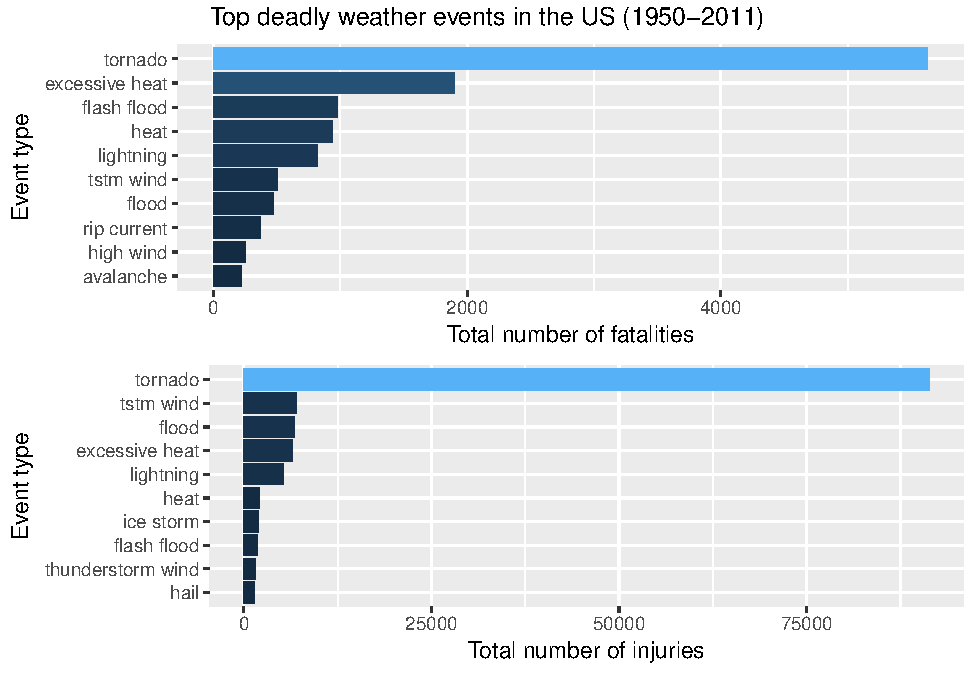
\includegraphics{storm_files/figure-latex/unnamed-chunk-11-1.pdf}

Tornadoes cause most number of deaths and injuries among all event
types. There are more than 5,000 deaths and more than 10,000 injuries in
the last 60 years in US, due to tornadoes. The other event types that
are most dangerous with respect to population health are excessive heat
and flash floods.

\subsection{Economic impact of weather
events}\label{economic-impact-of-weather-events}

The following plot shows the most severe weather event types with
respect to economic cost that they have costed since 1950s.

\begin{Shaded}
\begin{Highlighting}[]
\KeywordTok{library}\NormalTok{(ggplot2)}
\KeywordTok{library}\NormalTok{(gridExtra)}
\CommentTok{# Set the levels in order}
\NormalTok{p1 <-}\StringTok{ }\KeywordTok{ggplot}\NormalTok{(}\DataTypeTok{data=}\NormalTok{prop_dmg_events,}
             \KeywordTok{aes}\NormalTok{(}\DataTypeTok{x=}\KeywordTok{reorder}\NormalTok{(EVTYPE, prop_dmg), }\DataTypeTok{y=}\KeywordTok{log10}\NormalTok{(prop_dmg), }\DataTypeTok{fill=}\NormalTok{prop_dmg )) }\OperatorTok{+}
\StringTok{    }\KeywordTok{geom_bar}\NormalTok{(}\DataTypeTok{stat=}\StringTok{"identity"}\NormalTok{) }\OperatorTok{+}
\StringTok{    }\KeywordTok{coord_flip}\NormalTok{() }\OperatorTok{+}
\StringTok{    }\KeywordTok{xlab}\NormalTok{(}\StringTok{"Event type"}\NormalTok{) }\OperatorTok{+}
\StringTok{    }\KeywordTok{ylab}\NormalTok{(}\StringTok{"Property damage in dollars (log-scale)"}\NormalTok{) }\OperatorTok{+}
\StringTok{    }\KeywordTok{theme}\NormalTok{(}\DataTypeTok{legend.position=}\StringTok{"none"}\NormalTok{)}

\NormalTok{p2 <-}\StringTok{ }\KeywordTok{ggplot}\NormalTok{(}\DataTypeTok{data=}\NormalTok{crop_dmg_events,}
             \KeywordTok{aes}\NormalTok{(}\DataTypeTok{x=}\KeywordTok{reorder}\NormalTok{(EVTYPE, crop_dmg), }\DataTypeTok{y=}\NormalTok{crop_dmg, }\DataTypeTok{fill=}\NormalTok{crop_dmg)) }\OperatorTok{+}
\StringTok{    }\KeywordTok{geom_bar}\NormalTok{(}\DataTypeTok{stat=}\StringTok{"identity"}\NormalTok{) }\OperatorTok{+}
\StringTok{    }\KeywordTok{coord_flip}\NormalTok{() }\OperatorTok{+}\StringTok{ }
\StringTok{    }\KeywordTok{xlab}\NormalTok{(}\StringTok{"Event type"}\NormalTok{) }\OperatorTok{+}
\StringTok{    }\KeywordTok{ylab}\NormalTok{(}\StringTok{"Crop damage in dollars"}\NormalTok{) }\OperatorTok{+}\StringTok{ }
\StringTok{    }\KeywordTok{theme}\NormalTok{(}\DataTypeTok{legend.position=}\StringTok{"none"}\NormalTok{)}

\KeywordTok{grid.arrange}\NormalTok{(p1, p2, }\DataTypeTok{top=}\StringTok{"Weather costs to the US economy (1950-2011)"}\NormalTok{)}
\end{Highlighting}
\end{Shaded}

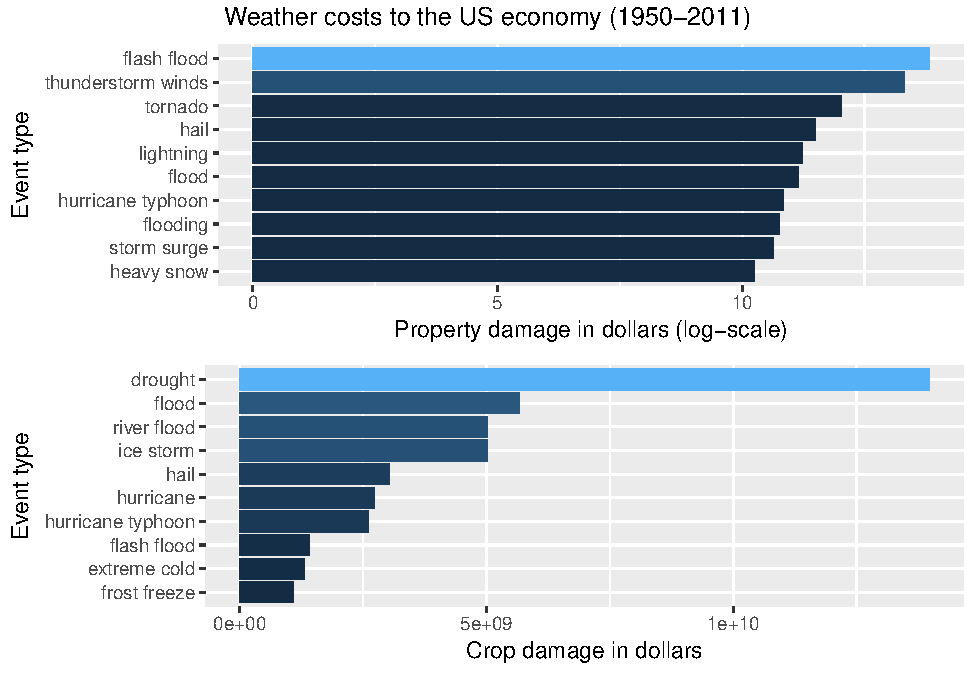
\includegraphics{storm_files/figure-latex/unnamed-chunk-12-1.pdf}

Property damages are given in logarithmic scale due to large range of
values. The data shows that flash floods and thunderstorm winds cost the
largest property damages among weather-related natural diseasters. Note
that, due to untidy nature of the available data, type \texttt{flood}
and \texttt{flash\ flood} are separate values and should be merged for
more accurate data-driven conclusions.

The most severe weather event in terms of crop damage is the drought. In
the last half century, the drought has caused more than 10 billion
dollars damage. Other severe crop-damage-causing event types are floods
and hails.


\end{document}
